\renewcommand{\theequation}{\theenumi}
\begin{enumerate}[label=\thesubsection.\arabic*.,ref=\thesubsection.\theenumi]
%\begin{enumerate}[label=\arabic*.,ref=\thesection.\theenumi]
\numberwithin{equation}{enumi}

\item Find the distance between the points 
\begin{align}
\myvec{0\\0}, \myvec{36\\15}
\end{align}
%
\solution The desired distance is 
\begin{align}
\norm{\vec{A} - \vec{B}} 
=\norm{\myvec{0\\0} - \myvec{36\\15}} = \sqrt{36^2+15^2} = 39
\end{align}

\item Find the distance between the following pairs of points
\begin{enumerate}
\item 
\begin{align}
\myvec{2\\3}, \myvec{4\\1}
\end{align}
\item 
\begin{align}
\myvec{-5\\7}, \myvec{-1\\3}
\end{align}
\item 
\begin{align}
\myvec{a\\b}, \myvec{-1\\b}
\end{align}
\end{enumerate}
\solution The distance between two vectors is given by 
\begin{align}
\norm{\vec{A}-\vec{B}}
\label{eq:vectors_3.5.1_norm}
\end{align}
From \eqref{eq:vectors_3.5.1_norm},
\begin{enumerate}
\item 
$\norm{\myvec{2\\3}-\myvec{4\\1}}=\sqrt{\brak{2-4}^2+\brak{3-1}^2 = 2\sqrt{2}}$
\item $\norm{\myvec{-5\\7}-\myvec{-1\\3}}=\sqrt{\brak{-5+1}^2+\brak{7-3}^2 = 4\sqrt{2}}$
\item $\norm{\myvec{a\\b}-\myvec{-1\\b}}=a+1$

\end{enumerate}
\item Name the type of quadrilateral formed, if any, by the following points, and give reasons for your answer.
\begin{enumerate}
\item 
\begin{align}
\vec{P} = \myvec{-1\\-2}, \vec{Q} =\myvec{1\\0},
\vec{R} =\myvec{-1\\2}, \vec{S} =\myvec{-3\\0}
\end{align}
\item 
\begin{align}
\vec{P} = \myvec{-3\\5}, \vec{Q} =\myvec{3\\1},
\vec{R} =\myvec{0\\3}, \vec{S} =\myvec{-1\\-4}
\end{align}
\item 
\begin{align}
\vec{P} = \myvec{4\\5}, \vec{Q} =\myvec{7\\6},
\\
\vec{R} =\myvec{4\\3}, \vec{S} =\myvec{1\\2}
\end{align}
\end{enumerate}
\solution
\begin{enumerate}
\item In Fig. 	\ref{fig:3.5.4_quadrilateral1}
\begin{align}
\label{eq:constr_vectors_quad1_PSQR}
 \vec{P} - \vec{S} &= 
 \vec{Q} - \vec{R} = \myvec{2\\-2}
\\
\vec {R} - \vec {S} &=
 \vec {Q} - \vec {P} = \myvec{2\\2}
\label{eq:constr_vectors_quad1_RSQP}
\end{align}
%
Hence $PQRS$ is a $\parallel$gm $\because$  opposite sides are parallel. Also, 
\begin{align}
\norm{ \vec{P} - \vec{S}} &= 
\norm{ \vec{Q} - \vec{R}} 
\\
=\norm{\vec {R} - \vec {S}} &=
\norm{ \vec {Q} - \vec {P}} = 2\sqrt{2}
\end{align}
%
$\because$ all sides are equal, the $\parallel$gm is a rhombus. The angle between $PS$ and
$RS$ is given by 
\begin{align}
\cos \theta = \frac{\brak{\vec{S}-\vec{P}}^{\top}\brak{\vec{S}-\vec{R}}}{\norm{\vec{S}-\vec{P}}^{\top}\norm{\vec{S}-\vec{R}}}
\end{align}
%
$\because $
\begin{align}
\brak{\vec{S}-\vec{P}}^{\top}\brak{\vec{S}-\vec{R}} = \myvec{2 & -2}\myvec{2\\2} = 0
\end{align}
upon substituting from \eqref{eq:constr_vectors_quad1_PSQR} and \eqref{eq:constr_vectors_quad1_RSQP}, 
\begin{align}
\cos \theta = 0 \implies PS \perp RS
\end{align}
%
Thus, the rhombus is actually a square.

\begin{figure}[!ht]
	\centering
	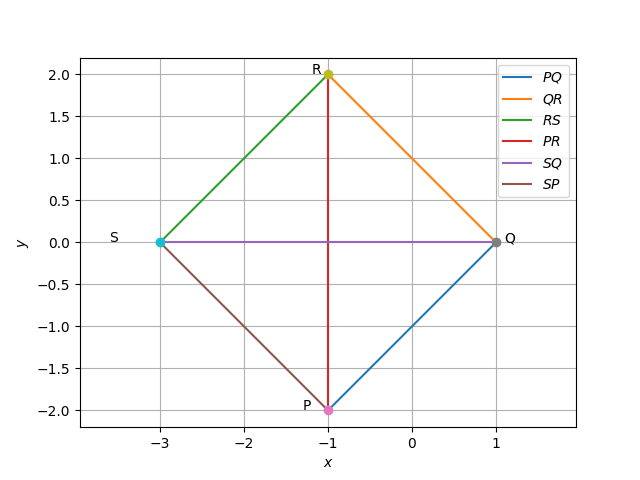
\includegraphics[width=\columnwidth]{./figs/vectors/quad1.png}
	\caption{quadrilateral1 }
	\label{fig:3.5.4_quadrilateral1}
\end{figure}
\begin{lstlisting}
codes/vectors/quad1.py
\end{lstlisting}

\item In Fig. 	\ref{fig:3.5.4_quadrilateral2}

\begin{align}
\vec{Q} - \vec{P} &= \myvec{6\\-4}
\\
\vec{R} - \vec{P} &= \myvec{3\\-2}
\\
\vec{Q} - \vec{R} &= \myvec{3\\-2}
\\
\left(\vec{Q} - \vec{P}\right) &= \left(\vec{R} - \vec{P}\right) + \left(\vec{Q} - \vec{R}\right) = \myvec{6\\-4}
\end{align}
Hence,  $\vec P,\vec Q$ and $\vec R$ lie on a straight line, so $PQRS$ is not  a quadrilateral.
%
\begin{figure}[!ht]
	\centering
	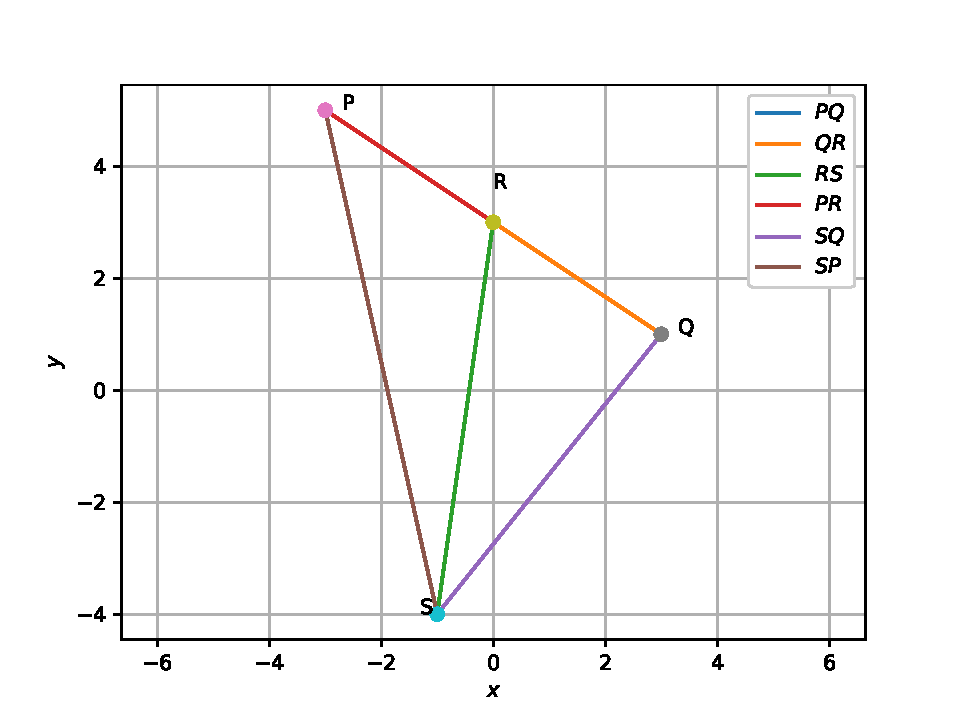
\includegraphics[width=\columnwidth]{./figs/vectors/quad2.pdf}
	\caption{quadrilateral2 }
	\label{fig:3.5.4_quadrilateral2}
\end{figure}
%
\item See Fig. 	\ref{fig:3.5.4_quadrilateral3}.

\begin{align}
\because \left(\vec{Q} - \vec{P}\right) &= \left(\vec{R} - \vec{S}\right) = \myvec{3\\1}
\\
\left(\vec{P} - \vec{S}\right) &= \left(\vec{Q} - \vec{R}\right) = \myvec{3\\3},
\end{align}
$PQRS$ is a parallelogram.  Also, 
%
\begin{align}
\norm{\vec{Q} - \vec{P}} \ne \norm{\vec{P} - \vec{S}}
\end{align}
Hence, $PQRS$ is neither a rhombus nor a square.
\begin{align}
\because \left(\vec{Q} - \vec{P}\right)^T \left(\vec{Q} - \vec{R}\right) = \myvec{3 & 1}\myvec{3\\3} \ne 0,
\end{align}
$PQRS$ is not a rectangle. 
%
\begin{figure}[!ht]
	\centering
	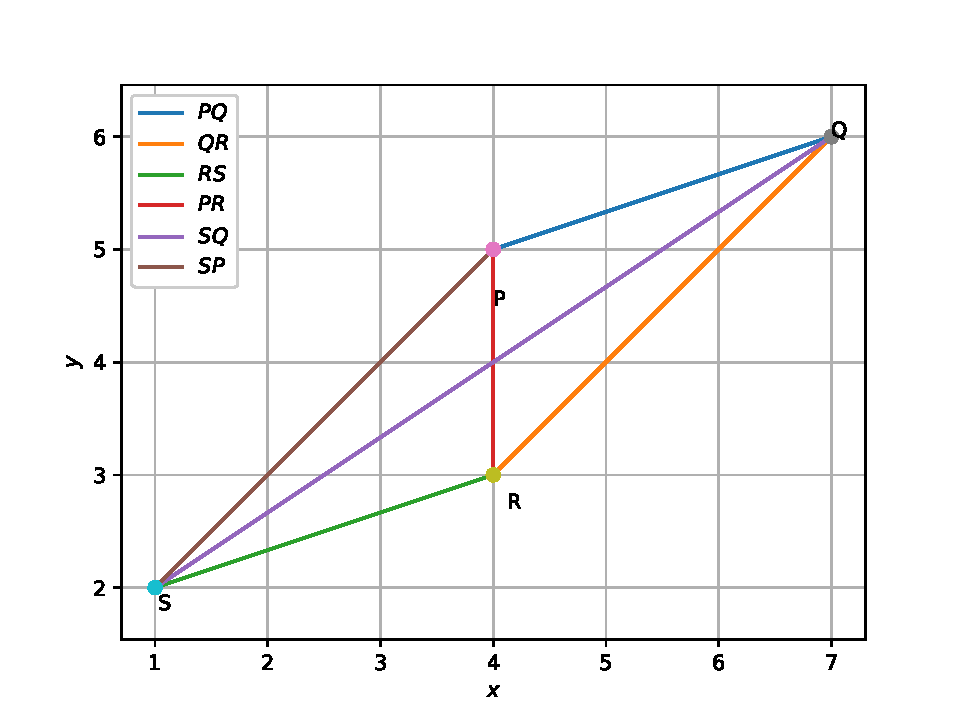
\includegraphics[width=\columnwidth]{./figs/vectors/quad3.pdf}
	\caption{}
	\label{fig:3.5.4_quadrilateral3}
\end{figure}

\end{enumerate}


\end{enumerate}
